\section{Experimental Details Behind Proteomic Data}
\label{sec:SI_exp_summary}
Here we provide a brief summary of the experiments behind each proteomic data
set considered. The purpose of this section is to identify how the authors
arrived at absolute protein abundances. In the following section
(see section on~\nameref{sec:SI_data_summary}) we will then provide a summary of the
protein abundance measurements. Table \ref{tab:datasets} provides an overview of
the publications we considered. These are predominately mass spectrometry-based,
with the exception of the work from \cite{li2014} which used ribosomal
profiling, and the fluorescence-based counting done in \cite{taniguchi2010}.
After having compiled and comparing these  measurements, we noted substantial
deviations in the measurements from \cite{taniguchi2010} and \cite{soufi2015}
(shown in the following section), and decided to only use the data from
\cite{schmidt2016, li2014, valgepea2013, peebo2015} in the main text. For
completeness, we include these additional datasets in our discussion of the experimental
data.

\begin{table}[bt]
\caption{\label{tab:datasets}Overview of proteomic data sets.}
\begin{tabular}{l l l }
\toprule
Author & Method & Reported Quantity \\
\midrule
Taniguchi \textit{et al.} (2010)  & YFP-fusion, cell fluorescence    & fg/copies per cell      \\
Valgepea \textit{et al.} (2012)   & mass spectrometry                & fg/copies per cell      \\
Peebo \textit{et al.} (2014)      & mass spectrometry                & fg/copies per fL        \\
Li \textit{et al.} (2014)         & ribosomal profiling              & fg/copies per cell $^a$ \\
Soufi \textit{et al.} (2015)      & mass spectrometry                & fg/copies per cell      \\
Schmidt \textit{et al.} (2016)    & mass spectrometry                & fg/copies per cell $^b$ \\
\bottomrule
\end{tabular}

\medskip
a. The reported values assume that the proteins are long-lived compared to the
generation time but are unable to account for post-translational modifications
that may alter absolute protein abundances.
\\
b. This mass spectrometry approach differs substantially from the others since
in addition to the relative proteome-wide abundance measurements, the authors
performed absolute quantification of 41 proteins across all growth conditions
(see section on~\nameref{sec:SI_schmidt} for more details on this).
\end{table}

\subsection{Fluorescence based measurements}
In the work of \cite{taniguchi2010}, the authors used a chromosomal YFP fusion
library where individual strains have a specific gene tagged with a YFP-coding
sequence. 1018 of their 1400 attempted strains were used in the work. A
fluorescence microscope was used to collect cellular YFP intensities across  all
these strains. Through automated image analysis, the authors normalized
intensity measurements by cell size to account for the change in size and
expression variability across the cell cycle. Following correction of  YFP
intensities for cellular autofluorescence, final absolute protein levels were
determined by a calibration curve with single-molecule fluorescence intensities.
This calibration  experiment was performed separately using a purified YFP
solution.

\subsection{Ribosomal profiling measurements}
The work of \cite{li2014} takes a sequencing based approach to estimate protein
abundance. Ribosomal profiling, which refers to the deep sequencing of
ribosome-protected mRNA fragments, can provide a quantitative measurement of the
protein synthesis rate.  As long as the protein life-time is long relative to
the cell doubling time, it is possible to  estimate absolute protein copy
numbers. The absolute protein synthesis rate has units of  proteins per generation,
and for stable proteins will also correspond to the protein  copy number per
cell.

In the experiments, ribosome-protected mRNA is extracted from cell lysate  and
selected on a denaturing polyacrylamide gel for deep sequencing (15–45 nt long
fragments collected and sequenced  by using an Illumina HiSeq 2000 in
\cite{li2014}). Counts of ribosome footprints from the sequencing data were then
corrected empirically for position-dependent biases in ribosomal density across
each gene, as well as dependencies on specific sequences including the
Shine-Dalgarno sequence. These data-corrected ribosome densities represent
relative protein synthesis rates. Absolute protein synthesis rates are obtained
by multiplying the relative rates by the total cellular protein per cell. The
total protein  per unit volume  was determined with the Lowry method to quantify
total protein, calibrated against bovine serum albumin (BSA). By counting
colony-forming units following serial dilution of their cell cultures, they then
calculated the total protein per cell.

\subsection{Mass spectrometry measurements}
Perhaps not surprisingly, the data is predominantly mass spectrometry based. This is
largely due to tremendous improvements in the sensitivity of mass spectrometers,
as well as improvements in sample preparation and data analysis
pipelines. It is now a relatively routine task to extract protein from a cell
and quantify the majority of proteins present by shotgun proteomics. In general, this
involves lysing cells, enzymatically digesting the proteins into short peptide
fragments, and then introducing them into the mass spectrometer (e.g.
with liquid chromatography and electrospray ionization), which itself can
have multiple rounds of detection and further fragmentation of the peptides.

Most quantitative experiments rely on labeling protein with stable isotopes,
which allow multiple samples to be measured together by the mass spectrometer.
By measuring samples of known total protein abundance simultaneously (i.e. one
sample of interest, and one reference), it is possible to determine relative
protein abundances. Absolute protein abundances can be estimated following the
same approach used above for ribosomal profiling, which is to multiply each
relative abundance measurement by the total cellular protein per cell. This is
the approach taken by \cite{valgepea2013, peebo2015} and \cite{soufi2015}, with
relative protein abundances determined based on the relative peptide intensities
(label free quantification 'LFQ' intensities). For the data of
\cite{valgepea2013}, total protein per cell was determined by measuring  total
protein by the Lowry method, and counting colony-forming units following serial
dilution. For the data from   \cite{peebo2015}, the authors did not determine
cell quantities and instead report the cellular protein abundances in protein
per unit  volume by assuming a mass density of 1.1 g/ml, with a 30\% dry mass
fraction.

An alternative way to arrive at absolute protein abundances is to dope in
synthetic peptide  fragments of known abundance. These can serve as a direct way
to calibrate mass spectrometry  signal intensities to absolute mass. This is the
approach taken by \cite{schmidt2016}. In addition  to a set of shotgun proteomic
measurements to determine proteome-wide relative abundances,  the authors also
performed absolute quantification of  41 proteins covering over four orders of
magnitude in cellular abundance. Here,  a synthetic peptide was generated for
each of the proteins, doped into each protein sample, and used these to
determine absolute protein abundances of the 41 proteins. These absolute
measurements, determined for every growth condition,  were then used as a
calibration curve to convert proteomic-wide relative abundances into  absolute
protein abundance per cell. A more extensive discussion of the
\cite{schmidt2016} data set can be found in Section \nameref{sec:SI_schmidt}.

\section{Summary of Proteomic Data}
\label{sec:SI_data_summary}
In the work of the main text we only used the data from \cite{valgepea2013,
li2014, peebo2015, schmidt2016}. As shown in \FIG{total_protein_final}(A), the
reported total protein abundances in the work of \cite{taniguchi2010} and
\cite{soufi2015} differed quite substantially from the other work. For the work
of \cite{taniguchi2010} this is in part due to a lower coverage in total
proteomic mass quantified, though we also noticed that most proteins appear
undercounted when compared to the other data.

\FIG{total_protein_final}(B) summarizes the total protein mass for each data
set used in our final compiled data set. Our inclination initally was to
leave reported copy numbers untouched, but a notable descrepency between the scaling
of the total protein per cell between \cite{schmidt2016} and the other data sets
forced us to dig deeper into those measurements (compare \cite{schmidt2016} and
\cite{li2014} data in \FIG{total_protein_final}(A)). The particular trend in
\cite{schmidt2016} appears to be due to assumptions made about cell size and we
provide a more extensive discussion and analysis of their data in
\nameref{sec:SI_schmidt}. As a compromise, and in an effort to treat all data
equally, we instead applied an correction factor to all protein abundance values
based on a data-driven estimate of total protein per cell. Here we used cell
size measurements from \cite{si2017, si2019}, and an estimate of total protein
content through expected dry mass. Total protein per cell was then determined
using available data on total DNA, RNA, and protein from \cite{basan2015,
dai2016}, which  account for the majority of dry mass in the cell. We describe
these details further in sections  on \nameref{sec:protein_size_SV} and
\nameref{sec:estimate_protein_per_cell} that follows.

\begin{figure}
    \begin{fullwidth}
    \centering{
        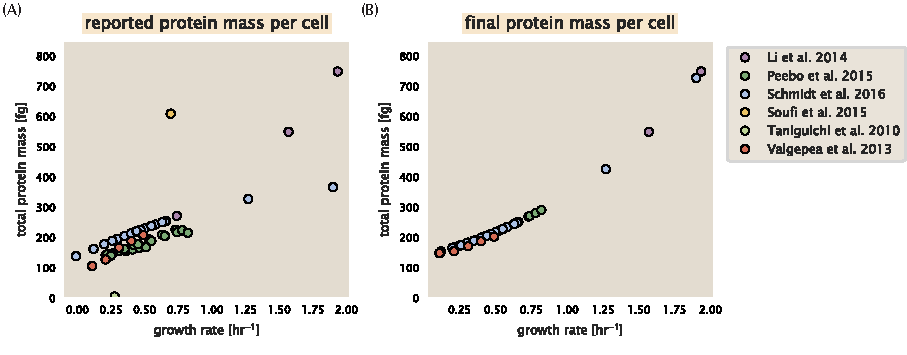
\includegraphics{SI_figs/figA1_dataset_corrections.pdf}
        \caption{\textbf{Summary of the growth-rate dependent total protein
        abundance for each data set.} (A) Total protein abundance per cell as
        originally reported in the data sets of \cite{taniguchi2010, valgepea2013, li2014,
        soufi2015, peebo2015, schmidt2016}. Note that the data from \cite{peebo2015} only
        reported protein abundances per unit volume and total protein per cell
        was found by multiplying these by the growth-rate dependent cell size as
        determined by \cite{si2017}. (B) Adjusted total protein abundances
        across the proteomic data sets are summarized. Protein abundances were
        adjusted so that all data shared a common set of growth-rate dependent
        total protein per cell and cellular protein concentration following the
        cell size expectations of \cite{si2017} (see section on
        \nameref{sec:protein_size_SV} for further details). }
        \label{fig:total_protein_final}
    }
    \end{fullwidth}
\end{figure}

Lastly, in \FIG{venn} we show the total proteomic coverage and overlap of
proteins quantified across each data set. In part (A) we plot the total number
of  unique proteins, while in part (B) we plot a Venn diagram to also show the
intersections across each data set. Overall, the overlap in quantified proteins
is quite high, with 1157 proteins quantified across all data sets. The
sequencing based approach of \cite{li2014} has substantially higher coverage
compared to the mass spectrometry data sets (3394 genes versus the 2041 genes
quantified in the work of \cite{schmidt2016}). However, in terms of total
protein mass, the data from \cite{li2014, schmidt2016, peebo2015} each quantify
roughly equivalent total protein mass.  An exception to this is in the data from
\cite{valgepea2013}, where we find that  the total protein quantified in
\cite{valgepea2013} is 90-95 \% of the total protein mass (when using the data
from \cite{schmidt2016} as a reference).


\begin{figure*}
    \centering{
        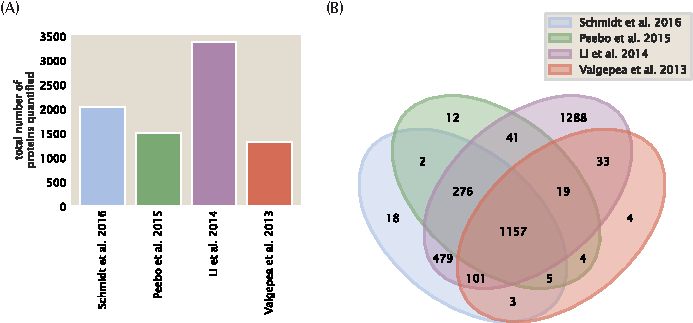
\includegraphics{SI_figs/figA2_intersections_venn.pdf}
        \caption{\textbf{Comparison of proteomic coverage across different data sets.}
        (A) Total number of unique proteins quantified in the data sets of
        \cite{valgepea2013, li2014, schmidt2016, peebo2015}. (2) Venn diagram
        showing the number of unique proteins and their intersections across each
        of the four data sets in (A). The intersection of all four data
        sets identifies 1157 proteins with measured protein copy number values. The
        intersection of each of the shaded colors identifies the number of
        unique proteins quantified only in those overlapping data sets.
        } \label{fig:venn}
    }
\end{figure*}
